\documentclass{standalone}

% graphics
\usepackage{tikz}
\usepackage{pgfplots}
\usepackage{siunitx}

\begin{document}

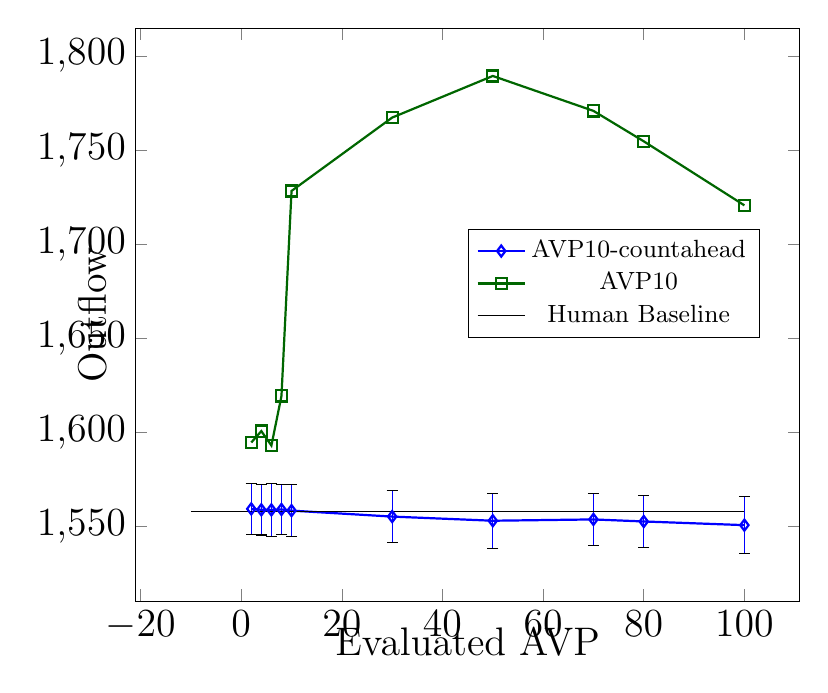
\begin{tikzpicture}[scale=1]
  \pgfplotsset{
      scale only axis,
      every x tick label/.append style={font=\Large},
      every y tick label/.append style={font=\Large},
	legend style={at={(0.5,0.65)},anchor=north west}
  }

\begin{axis}[
    legend style={font=\small},
	ylabel={\Large Outflow},
	x label style={at={(axis description cs:0.5,-0.03)},anchor=north},
	y label style={at={(axis description cs:-0.030,0.5)}, anchor=south},
	xlabel={\Large Evaluated AVP},
]




% trained on avp=10 
% dashdotdotted,
\addplot[mark=diamond, thick, mark options={solid, fill=blue!40, mark size=2 pt}, draw=blue, error bars/.cd, y dir=both, y explicit] table [x=a, y=b, y error=c] {
a	b   	c
2 1559.48 13.64
4 1558.98 13.35
6 1558.94 13.95
8 1559.16 13.39
10 1558.55 13.87
30 1555.38 13.85
50 1553.18 14.63
70 1553.87 13.93
80 1552.79 13.60
100 1550.84 14.98
};
\label{AVP10-countahead}

% trained on avp=30
% error bars/.cd, y dir=both, y explicit,
\addplot[mark=square, thick, mark options={solid, fill=green!60, mark size=2 pt}, draw=black!60!green] table [x=a, y=b] {
a	b   	c
2	1594.73	20.77
4 	1600.78 21.92	
6	1593.11 20.44
8	1619.46 27.24
10	1728.32 30.39
30 	1767.28 46.92
50	1789.38 39.06
70	1770.84 36.94
80	1754.68 29.82
100	1720.66 27.16
};
\label{AVP10}  

\addplot[mark=none, black, samples=200] coordinates {(-10,1558.12)
(100,1558.12)};
\label{Baseline}


\addlegendimage{/pgfplots/refstyle=AVP10}
\addlegendentry{AVP10-countahead}

\addlegendimage{/pgfplots/refstyle=AVP30}
\addlegendentry{AVP10}

%\addlegendimage{/pgfplots/refstyle=linearPPO}
%\addlegendentry{linearPPOAVP10}

\addlegendimage{/pgfplots/refstyle=Baseline}
\addlegendentry{Human Baseline}




\end{axis}
\end{tikzpicture}

\end{document}

